%%%%%%%%%%%%%%%%%%%%%%%%%%%%%%%%%%%%%%%%%
% Classicthesis Typographic Thesis
% LaTeX Template
% Version 1.3 (15/2/14)
%
% This template has been downloaded from:
% http://www.LaTeXTemplates.com
%
% Original author:
% André Miede (http://www.miede.de)
%
% License:
% CC BY-NC-SA 3.0 (http://creativecommons.org/licenses/by-nc-sa/3.0/)
%
% General Tips:
% 1) Make sure to edit the classicthesis-config.file
% 2) New enumeration (A., B., C., etc in small caps): \begin{aenumerate} \end{aenumerate}
% 3) For margin notes: \marginpar or \graffito{}
% 4) Do not use bold fonts in this style, it is designed around them
% 5) Use tables as in the examples
% 6) See classicthesis-preamble.sty for useful commands
%
%%%%%%%%%%%%%%%%%%%%%%%%%%%%%%%%%%%%%%%%%

%----------------------------------------------------------------------------------------
%	PACKAGES AND OTHER DOCUMENT CONFIGURATIONS
%----------------------------------------------------------------------------------------

\documentclass[
		twoside,openright,titlepage,numbers=noenddot,headinclude,%1headlines,
                footinclude=true,cleardoublepage=empty,
                BCOR=5mm,paper=a4,fontsize=11pt, % Binding correction, paper type and font size
                ngerman,american, % Languages
                ]{scrreprt} 
                
% Includes the file which contains all the document configurations and packages - make sure to edit this file
%----------------------------------------------------------------------------------------
%	DOCUMENT VARIABLES
%	Fill in the lines below to enter your information into the thesis template
%	Each of the commands can be cited anywhere in the thesis
%----------------------------------------------------------------------------------------

% Remove drafting to get rid of the '[ Date - classicthesis version 4.0 ]' text at the bottom of every page
\PassOptionsToPackage{
	eulerchapternumbers,
	listings,pdfspacing, 
	subfig,
	beramono,
	eulermath,
	parts
}{classicthesis}
% Available options: drafting parts nochapters linedheaders eulerchapternumbers beramono eulermath pdfspacing minionprospacing tocaligned dottedtoc manychapters listings floatperchapter subfig
% Adding 'dottedtoc' will make page numbers in the table of contents flushed right with dots leading to them

\newcommand{\myTitle}{Smart gateway for Low-Power Lossy Networks\xspace}
\newcommand{\mySubtitle}{A PhD thesis\xspace}
\newcommand{\myDegree}{Doktor-Ingenieur (Dr.-Ing.)\xspace}
\DeclareRobustCommand{\myName}{Remy Leone\xspace}
\newcommand{\myProf}{Put name here\xspace}
\newcommand{\myOtherProf}{Put name here\xspace}

\newcommand{\Paolo}{Dr. Paolo MEDAGLIANI\xspace}
\newcommand{\Jeremie}{Dr. Jeremie LEGUAY\xspace}
\newcommand{\Claude}{Dr. Claude CHAUDET\xspace}
\newcommand{\Vania}{Dr. Vania CONAN\xspace}
\newcommand{\JeanLouis}{Dr. Jean Louis ROUGIER\xspace}

\newcommand{\myFaculty}{Put data here\xspace}
\newcommand{\myDepartment}{Put data here\xspace}
\newcommand{\myUni}{Telecom Paris Tech\xspace}
\newcommand{\myLocation}{Paris, France\xspace}
\newcommand{\myTime}{\today\xspace}
\newcommand{\myVersion}{version 4.0\xspace}

%----------------------------------------------------------------------------------------
%	USEFUL COMMANDS
%----------------------------------------------------------------------------------------

\newcommand{\ie}{i.\,e.}
\newcommand{\Ie}{I.\,e.}
\newcommand{\eg}{e.\,g.}
\newcommand{\Eg}{E.\,g.} 

\newcounter{dummy} % Necessary for correct hyperlinks (to index, bib, etc.)
\providecommand{\mLyX}{L\kern-.1667em\lower.25em\hbox{Y}\kern-.125emX\@}

%----------------------------------------------------------------------------------------
%	PACKAGES
%----------------------------------------------------------------------------------------

\usepackage{lipsum} % Used for inserting dummy 'Lorem ipsum' text into the template

%------------------------------------------------
 
\PassOptionsToPackage{utf8}{inputenc} % latin9 (ISO-8859-9) = latin1+"Euro sign"
\usepackage{inputenc}
 
 %------------------------------------------------

%\usepackage[francais]{babel}

%------------------------------------------------			

% \PassOptionsToPackage{square,numbers}{natbib}
%  \usepackage{natbib}

\usepackage{multibib} % option to reset the bib item numbering
\newcites{mine}{My Publications}
% \usepackage[
%     style=numeric-comp,
%     bibstyle=numeric,
%     sorting=none,
%     url=false,
%     natbib=true,
%     backend=biber
% ]{biblatex} % Load the package with some options.
% \addbibresource{Bibliography.bib}

 %------------------------------------------------

\PassOptionsToPackage{fleqn}{amsmath} % Math environments and more by the AMS 
 \usepackage{amsmath}

 %------------------------------------------------

\PassOptionsToPackage{T1}{fontenc} % T2A for cyrillics
\usepackage{fontenc}

%------------------------------------------------

\usepackage{xspace} % To get the spacing after macros right

%------------------------------------------------

\usepackage{mparhack} % To get marginpar right

%------------------------------------------------

\usepackage{fixltx2e} % Fixes some LaTeX stuff 

%------------------------------------------------

\PassOptionsToPackage{smaller}{acronym} % Include printonlyused in the first bracket to only show acronyms used in the text
\usepackage{acronym} % nice macros for handling all acronyms in the thesis

%------------------------------------------------

%\renewcommand*{\acsfont}[1]{\textssc{#1}} % For MinionPro
\renewcommand{\bflabel}[1]{{#1}\hfill} % Fix the list of acronyms

%------------------------------------------------

\PassOptionsToPackage{pdftex}{graphicx}
\usepackage{graphicx} 

%------------------------------------------------
% Static Analysis of LaTeX source code
%------------------------------------------------
\RequirePackage[l2tabu, orthodox]{nag}

%------------------------------------------------
% Telecom Paris Tech
%------------------------------------------------

\usepackage{geometry}
\usepackage{eso-pic}
\usepackage{ifpdf}

\newcommand\BackgroundPicLastPage{
\ifpdf
	
\includegraphics[height=\paperheight,width=\paperwidth]{img/logos/cover_4_bg.pdf}
\else
	
\includegraphics[height=\paperheight,width=\paperwidth]{img/logos/cover_4_bg.pdf}
\fi
}


\newcommand\BackgroundPicCover{
\ifpdf
	
\includegraphics[height=\paperheight,width=\paperwidth]{img/logos/cover_bg.pdf}
\else
	
\includegraphics[height=\paperheight,width=\paperwidth]{img/logos/cover_bg.pdf}
\fi}

%----------------------------------------------------------------------------------------
%	FLOATS: TABLES, FIGURES AND CAPTIONS SETUP
%----------------------------------------------------------------------------------------

\usepackage{tabularx} % Better tables
\setlength{\extrarowheight}{3pt} % Increase table row height
\newcommand{\tableheadline}[1]{\multicolumn{1}{c}{\spacedlowsmallcaps{#1}}}
\newcommand{\myfloatalign}{\centering} % To be used with each float for alignment
\usepackage{caption}
\captionsetup{format=hang,font=small}
\usepackage{subfig}  

%----------------------------------------------------------------------------------------
%	CODE LISTINGS SETUP
%----------------------------------------------------------------------------------------

\usepackage{listings} 
%\lstset{emph={trueIndex,root},emphstyle=\color{BlueViolet}}%\underbar} % for special keywords
\lstset{language=[LaTeX]Tex, % Specify the language for listings here
keywordstyle=\color{RoyalBlue}, % Add \bfseries for bold
basicstyle=\small\ttfamily, % Makes listings a smaller font size and a different font
%identifierstyle=\color{NavyBlue}, % Color of text inside brackets
commentstyle=\color{Green}\ttfamily, % Color of comments
stringstyle=\rmfamily, % Font type to use for strings
numbers=left, % Change left to none to remove line numbers
numberstyle=\scriptsize, % Font size of the line numbers
stepnumber=5, % Increment of line numbers
numbersep=8pt, % Distance of line numbers from code listing
showstringspaces=false, % Sets whether spaces in strings should appear underlined
breaklines=true, % Force the code to stay in the confines of the listing box
%frameround=ftff, % Uncomment for rounded frame
frame=single, % Frame border - none/leftline/topline/bottomline/lines/single/shadowbox/L
belowcaptionskip=.75\baselineskip % Space after the "Listing #: Desciption" text and the listing box
}

%----------------------------------------------------------------------------------------
%	HYPERREFERENCES
%----------------------------------------------------------------------------------------

\PassOptionsToPackage{pdftex,hyperfootnotes=false,pdfpagelabels}{hyperref}
\usepackage{hyperref}  % backref linktocpage pagebackref
\pdfcompresslevel=9
\pdfadjustspacing=1

\hypersetup{
% Uncomment the line below to remove all links (to references, figures, tables, etc)
%draft, 
colorlinks=true, linktocpage=true, pdfstartpage=3, pdfstartview=FitV,
% Uncomment the line below if you want to have black links (e.g. for printing black and white)
%colorlinks=false, linktocpage=false, pdfborder={0 0 0}, pdfstartpage=3, pdfstartview=FitV, 
breaklinks=true, pdfpagemode=UseNone, pageanchor=true, pdfpagemode=UseOutlines,
plainpages=false, bookmarksnumbered, bookmarksopen=true, bookmarksopenlevel=1,
hypertexnames=true, pdfhighlight=/O, urlcolor=webbrown, linkcolor=RoyalBlue, citecolor=webgreen,
%------------------------------------------------
% PDF file meta-information
pdftitle={\myTitle},
pdfauthor={\textcopyright\ \myName, \myUni, \myFaculty},
pdfsubject={},
pdfkeywords={},
pdfcreator={pdfLaTeX},
pdfproducer={LaTeX with hyperref and classicthesis}
%------------------------------------------------
}   

%----------------------------------------------------------------------------------------
%	BACKREFERENCES
%----------------------------------------------------------------------------------------

\usepackage{ifthen} % Allows the user of the \ifthenelse command
\newboolean{enable-backrefs} % Variable to enable backrefs in the bibliography
\setboolean{enable-backrefs}{true} % Variable value: true or false

\newcommand{\backrefnotcitedstring}{\relax} % (Not cited.)
\newcommand{\backrefcitedsinglestring}[1]{(Cited on page~#1.)}
\newcommand{\backrefcitedmultistring}[1]{(Cited on pages~#1.)}
\ifthenelse{\boolean{enable-backrefs}} % If backrefs were enabled
{
\PassOptionsToPackage{hyperpageref}{backref}
\usepackage{backref} % to be loaded after hyperref package 
\renewcommand{\backreftwosep}{ and~} % separate 2 pages
\renewcommand{\backreflastsep}{, and~} % separate last of longer list
\renewcommand*{\backref}[1]{}  % disable standard
\renewcommand*{\backrefalt}[4]{% detailed backref
\ifcase #1 
\backrefnotcitedstring
\or
\backrefcitedsinglestring{#2}
\else
\backrefcitedmultistring{#2}
\fi}
}{\relax} 

%----------------------------------------------------------------------------------------
%	AUTOREFERENCES SETUP
%	Redefines how references in text are prefaced for different 
%	languages (e.g. "Section 1.2" or "section 1.2")
%----------------------------------------------------------------------------------------

\makeatletter
\@ifpackageloaded{babel}
{
\addto\extrasamerican{
\renewcommand*{\figureautorefname}{Figure}
\renewcommand*{\tableautorefname}{Table}
\renewcommand*{\partautorefname}{Part}
\renewcommand*{\chapterautorefname}{Chapter}
\renewcommand*{\sectionautorefname}{Section}
\renewcommand*{\subsectionautorefname}{Section}
\renewcommand*{\subsubsectionautorefname}{Section}
}
\addto\extrasngerman{
\renewcommand*{\paragraphautorefname}{Absatz}
\renewcommand*{\subparagraphautorefname}{Unterabsatz}
\renewcommand*{\footnoteautorefname}{Fu\"snote}
\renewcommand*{\FancyVerbLineautorefname}{Zeile}
\renewcommand*{\theoremautorefname}{Theorem}
\renewcommand*{\appendixautorefname}{Anhang}
\renewcommand*{\equationautorefname}{Gleichung}
\renewcommand*{\itemautorefname}{Punkt}
}
\providecommand{\subfigureautorefname}{\figureautorefname} % Fix to getting autorefs for subfigures right
}{\relax}
\makeatother

%----------------------------------------------------------------------------------------

\usepackage{classicthesis} 

%----------------------------------------------------------------------------------------
%	CHANGING TEXT AREA 
%----------------------------------------------------------------------------------------

%\linespread{1.05} % a bit more for Palatino
%\areaset[current]{312pt}{761pt} % 686 (factor 2.2) + 33 head + 42 head \the\footskip
%\setlength{\marginparwidth}{7em}%
%\setlength{\marginparsep}{2em}%

%----------------------------------------------------------------------------------------
%	USING DIFFERENT FONTS
%----------------------------------------------------------------------------------------

% \usepackage[oldstylenums]{kpfonts} % oldstyle notextcomp
% \usepackage[osf]{libertine}
% \usepackage[light,condensed,math]{iwona}

% \usepackage[bitstream-charter]{mathdesign}
% \usepackage[urw-garamond]{mathdesign} <-- no osf support :-(


\begin{document}

\frenchspacing % Reduces space after periods to make text more compact

\raggedbottom % Makes all pages the height of the text on that page

%\selectlanguage{francais} % Select your default language - e.g. american or ngerman

%\renewcommand*{\bibname}{new name} % Uncomment to change the name of the bibliography
%\setbibpreamble{} % Uncomment to include a preamble to the bibliography - some text before the reference list starts

\pagenumbering{roman} % Roman page numbering prior to the start of the thesis content (i, ii, iii, etc)

\pagestyle{plain} % Suppress headers for the pre-content pages

%----------------------------------------------------------------------------------------
%	PRE-CONTENT THESIS PAGES
%----------------------------------------------------------------------------------------

%\documentclass[11pt,a4paper]{book}
%\usepackage[left=1.3cm,top=0cm,right=1.3cm,bottom=1.2cm]{geometry}

%\usepackage{textcomp}
%\usepackage{helvet}	% or \usepackage{lmodern}
%\renewcommand\textnumero{n$^{\textsf{{\tiny O}}}$}
%\renewcommand{\familydefault}{\sfdefault}

\newgeometry{left=1.3cm,top=0cm,right=1.3cm,bottom=1.2cm}

\pagestyle{empty}

\AddToShipoutPicture*{\BackgroundPicCover}

\begin{flushright}


\includegraphics[scale=0.3]{img/logos/telecom.eps}

{\small {2013-ENST-00xx~~~~}}

\end{flushright}

\vspace{0.cm}
\begin{center}


\includegraphics[scale=0.65]{img/logos/edite.eps} \\
{\small {EDITE - ED 130}}


\vspace{.5cm}

%{\Large École doctorale \textnumero XX: texte}\\		% version une ligne
%{\Large École doctorale \textnumero XX:\\ texte}\\		% version deux lignes (changer les espaces en conséquence

\vspace{1.0cm}

{\LARGE \textbf{Doctorat ParisTech}}\\
\vspace{1.1cm}
{\LARGE \textbf{T H È S E}}\\
\vspace{0.5cm}
{\normalsize \textbf{pour obtenir le grade de docteur délivré par}}\\

\vspace{.9cm}

{\LARGE \textbf{TELECOM ParisTech}}\\
\vspace{0.6cm}
{\Large \textbf{Spécialité Informatique et Réseaux}}\\

\vspace{.8cm}

{\normalsize \textit{présentée et soutenue publiquement par}}\\
\vspace{0.7cm}

{\Large \textbf{Remy LEONE}}\\
\vspace{0.24cm}
{\normalsize \today}\\

\vfill

\textcolor[RGB]{191,18,56}{
\noindent
{\LARGE \textbf{\myTitle}}\\
}

\vfill~\vfill

{\normalsize
\begin{tabular}{c}
Directeur de thèse: 			\textbf{\JeanLouis}\\
Co-encadrement de la thèse:		\textbf{\Vania}
\end{tabular}
}
\end{center}

\vfill

\flushleft
\begin{minipage}{.9\textwidth}	% ou .91\textwidth si vous n'avez pas assez de place
  \textbf{Jury}\\
% Mme/M. Prénom NOM, Titre, Unité de recherche, Ecole 

\textbf{\JeanLouis}, {\small Professeur, Télécom ParisTech, France}
	\hfill Directeur de thèse\\
\textbf{\Vania}, {\small Thales Communications \& Security}
	\hfill Directeur de thèse\\
\textbf{\Paolo}, {\small Huawei Technologies Co. Ltd.}
	\hfill Encadrant de thèse\\
\textbf{\Jeremie}, {\small Huawei Technologies Co. Ltd.}
	\hfill Encadrant de thèse\\
\textbf{\Claude}, {\small Maître de Conférences, Télécom ParisTech, France}
	\hfill Encadrant de thèse\\
\textbf{M. HODOR}, {\small Hodor}
	\hfill Hodor\\
\textbf{M. Chuck NORRIS}, {\small Titre, Unité de recherche, Ecole}
	\hfill Last Judge\\
\textbf{Mme Margaret THATCHER}, {\small Titre, Unité de recherche, Ecole}
	\hfill Examinatrice farouche\\

\end{minipage}\\

\vspace{-.3cm}

\centering
\textbf{TELECOM ParisTech}\\
{\small école de l'Institut Mines-Télécom - membre de ParisTech}\\
{\tiny 46 rue Barrault 75013 Paris - (+33) 1 45 81 77 77 - www.telecom-paristech.fr}

\restoregeometry


% Back of the title page

\thispagestyle{empty}

This thesis was financed by CIFRE project


\includegraphics[scale=0.2]{img/logos/telecom.eps}

\includegraphics[scale=0.2]{img/logos/thales.jpg}

\includegraphics[scale=0.12]{img/logos/lincs_pupuce.png}

\vfill

\noindent\myName: \textit{\myTitle,} \mySubtitle, %\myDegree, 
\textcopyright\ \myTime

% You may wish to do something with the back of the title page, such as including your supervisors, location or time frame of the work. Below is an example of doing so although you may want to tweak it to your liking.

\bigskip

\noindent\spacedlowsmallcaps{Supervisors}: \\
\Claude \\
\Jeremie \\ 
\Paolo \\
 % Back of the title page

\cleardoublepage% Dedication

\thispagestyle{empty}
\refstepcounter{dummy}

\pdfbookmark[1]{Dedication}{Dedication} % Bookmark name visible in a PDF viewer

\vspace*{3cm}

\begin{center}
\emph{Ohana} means family. \\
Family means nobody gets left behind, or forgotten. \\ \medskip
--- Lilo \& Stitch    
\end{center}

\medskip

\begin{center}
Dedicated to the loving memory of Rudolf Miede. \\ \smallskip
1939\,--\,2005
\end{center} % Dedication page

%\cleardoublepage\include{tex/Foreword} % Uncomment and create a Foreword.tex to include a foreword

\cleardoublepage% Abstract

\pdfbookmark[1]{Abstract}{Abstract} % Bookmark name visible in a PDF viewer

\begingroup
\let\clearpage\relax
\let\cleardoublepage\relax
\let\cleardoublepage\relax

\chapter*{Abstract} % Abstract name

Lorem ipsum dolor sit amet, consectetur adipisicing elit, sed do eiusmod
tempor incididunt ut labore et dolore magna aliqua. Ut enim ad minim veniam,
quis nostrud exercitation ullamco laboris nisi ut aliquip ex ea commodo
consequat. Duis aute irure dolor in reprehenderit in voluptate velit esse
cillum dolore eu fugiat nulla pariatur. Excepteur sint occaecat cupidatat non
proident, sunt in culpa qui officia deserunt mollit anim id est laborum.

\bigskip

Lorem ipsum dolor sit amet, consectetur adipisicing elit, sed do eiusmod
tempor incididunt ut labore et dolore magna aliqua. Ut enim ad minim veniam,
quis nostrud exercitation ullamco laboris nisi ut aliquip ex ea commodo
consequat. Duis aute irure dolor in reprehenderit in voluptate velit esse
cillum dolore eu fugiat nulla pariatur. Excepteur sint occaecat cupidatat non
proident, sunt in culpa qui officia deserunt mollit anim id est laborum.

Lorem ipsum dolor sit amet, consectetur adipisicing elit, sed do eiusmod
tempor incididunt ut labore et dolore magna aliqua. Ut enim ad minim veniam,
quis nostrud exercitation ullamco laboris nisi ut aliquip ex ea commodo
consequat. Duis aute irure dolor in reprehenderit in voluptate velit esse
cillum dolore eu fugiat nulla pariatur. Excepteur sint occaecat cupidatat non
proident, sunt in culpa qui officia deserunt mollit anim id est laborum.

Lorem ipsum dolor sit amet, consectetur adipisicing elit, sed do eiusmod
tempor incididunt ut labore et dolore magna aliqua. Ut enim ad minim veniam,
quis nostrud exercitation ullamco laboris nisi ut aliquip ex ea commodo
consequat. Duis aute irure dolor in reprehenderit in voluptate velit esse
cillum dolore eu fugiat nulla pariatur. Excepteur sint occaecat cupidatat non
proident, sunt in culpa qui officia deserunt mollit anim id est laborum.

\endgroup			

\vfill % Abstract page

\cleardoublepage% Publications - a page listing research articles written using content in the thesis

% \pdfbookmark[1]{Publications}{Publications} % Bookmark name visible in a PDF viewer

% \chapter*{Publications} % Publications page text

% Some ideas and figures have appeared previously in the following publications:

% \bigskip

% \noindent Put your publications from the thesis here. The packages
% \texttt{multibib} or \texttt{bibtopic} etc. can be used to handle multiple
% different bibliographies in your document.

% \nocitesec{*}

% \bibliographystylesec{plain}
% \bibliographysec{bib/mypublications}


% Print your own papers.
%\begin{refsection}
%% If you print a bibliography within this section, only citations within this refsection will be printed.
%
%% Option 1: Make nocite for all of your papers.
%% Options 2 would be a seperate file which contains all of your papers.
%
%\nocite{leone2013optimizing}
%
%\defbibnote{myPrenote}{
%    Some words before I show you the list of my own papers.
%}
%\defbibnote{myPostnote}{
%    A bunch of papers are still in print and not yet published.
%}
%\printbibliography[
%    heading=bibintoc,
%    title={Author's Contributions},
%    prenote=myPrenote,
%    postnote=myPostnote
%]
%\end{refsection}
 % Publications from the thesis page

\cleardoublepage% Acknowledgements

\pdfbookmark[1]{Acknowledgements}{Acknowledgements} % Bookmark name visible in a PDF viewer

% \begin{flushright}{\slshape    
% We have seen that computer programming is an art, \\ 
% because it applies accumulated knowledge to the world, \\ 
% because it requires skill and ingenuity, and especially \\
% because it produces objects of beauty.} \\ \medskip
% %--- \defcitealias{knuth:1974}{Donald E. Knuth}\citetalias{knuth:1974} \citep{knuth:1974}
% \end{flushright}

% \bigskip

%----------------------------------------------------------------------------------------

\begingroup

\let\clearpage\relax
\let\cleardoublepage\relax
\let\cleardoublepage\relax

\chapter*{Acknowledgements} % Acknowledgements section text

Lorem ipsum dolor sit amet, consectetur adipisicing elit, sed do eiusmod
tempor incididunt ut labore et dolore magna aliqua. Ut enim ad minim veniam,
quis nostrud exercitation ullamco laboris nisi ut aliquip ex ea commodo
consequat. Duis aute irure dolor in reprehenderit in voluptate velit esse
cillum dolore eu fugiat nulla pariatur. Excepteur sint occaecat cupidatat non
proident, sunt in culpa qui officia deserunt mollit anim id est laborum.

\bigskip

Lorem ipsum dolor sit amet, consectetur adipisicing elit, sed do eiusmod
tempor incididunt ut labore et dolore magna aliqua. Ut enim ad minim veniam,
quis nostrud exercitation ullamco laboris nisi ut aliquip ex ea commodo
consequat. Duis aute irure dolor in reprehenderit in voluptate velit esse
cillum dolore eu fugiat nulla pariatur. Excepteur sint occaecat cupidatat non
proident, sunt in culpa qui officia deserunt mollit anim id est laborum.

\bigskip

Lorem ipsum dolor sit amet, consectetur adipisicing elit, sed do eiusmod
tempor incididunt ut labore et dolore magna aliqua. Ut enim ad minim veniam,
quis nostrud exercitation ullamco laboris nisi ut aliquip ex ea commodo
consequat. Duis aute irure dolor in reprehenderit in voluptate velit esse
cillum dolore eu fugiat nulla pariatur. Excepteur sint occaecat cupidatat non
proident, sunt in culpa qui officia deserunt mollit anim id est laborum.

\bigskip

Lorem ipsum dolor sit amet, consectetur adipisicing elit, sed do eiusmod
tempor incididunt ut labore et dolore magna aliqua. Ut enim ad minim veniam,
quis nostrud exercitation ullamco laboris nisi ut aliquip ex ea commodo
consequat. Duis aute irure dolor in reprehenderit in voluptate velit esse
cillum dolore eu fugiat nulla pariatur. Excepteur sint occaecat cupidatat non
proident, sunt in culpa qui officia deserunt mollit anim id est laborum.

\endgroup % Acknowledgements page

\pagestyle{scrheadings} % Show chapter titles as headings

\cleardoublepage% Table of Contents - List of Tables/Figures/Listings and Acronyms

\refstepcounter{dummy}

\pdfbookmark[1]{\contentsname}{tableofcontents} % Bookmark name visible in a PDF viewer

\setcounter{tocdepth}{2} % Depth of sections to include in the table of contents - currently up to subsections

\setcounter{secnumdepth}{3} % Depth of sections to number in the text itself - currently up to subsubsections

\manualmark
\markboth{\spacedlowsmallcaps{\contentsname}}{\spacedlowsmallcaps{\contentsname}}
\tableofcontents 
\automark[section]{chapter}
\renewcommand{\chaptermark}[1]{\markboth{\spacedlowsmallcaps{#1}}{\spacedlowsmallcaps{#1}}}
\renewcommand{\sectionmark}[1]{\markright{\thesection\enspace\spacedlowsmallcaps{#1}}}

\clearpage

\begingroup 
\let\clearpage\relax
\let\cleardoublepage\relax
\let\cleardoublepage\relax

%----------------------------------------------------------------------------------------
%	List of Figures
%----------------------------------------------------------------------------------------

\refstepcounter{dummy}
%\addcontentsline{toc}{chapter}{\listfigurename} % Uncomment if you would like the list of figures to appear in the table of contents
\pdfbookmark[1]{\listfigurename}{lof} % Bookmark name visible in a PDF viewer

\listoffigures

\vspace*{8ex}
\newpage

%----------------------------------------------------------------------------------------
%	List of Tables
%----------------------------------------------------------------------------------------

% \refstepcounter{dummy}
% %\addcontentsline{toc}{chapter}{\listtablename} % Uncomment if you would like the list of tables to appear in the table of contents
% \pdfbookmark[1]{\listtablename}{lot} % Bookmark name visible in a PDF viewer

% \listoftables
        
% \vspace*{8ex}
% \newpage
    
%----------------------------------------------------------------------------------------
%	List of Listings
%---------------------------------------------------------------------------------------- 

% \refstepcounter{dummy}
% %\addcontentsline{toc}{chapter}{\lstlistlistingname} % Uncomment if you would like the list of listings to appear in the table of contents
% \pdfbookmark[1]{\lstlistlistingname}{lol} % Bookmark name visible in a PDF viewer

% \lstlistoflistings 

% \vspace*{8ex}
% \newpage
       
%----------------------------------------------------------------------------------------
%	Acronyms
%----------------------------------------------------------------------------------------

\refstepcounter{dummy}
%\addcontentsline{toc}{chapter}{Acronyms} % Uncomment if you would like the acronyms to appear in the table of contents
\pdfbookmark[1]{Acronyms}{acronyms} % Bookmark name visible in a PDF viewer

\markboth{\spacedlowsmallcaps{Acronyms}}{\spacedlowsmallcaps{Acronyms}}

% USE \ac{my_acronym} to have it reference.

\chapter*{Acronyms}

\begin{acronym}[UML]
\acro{DRY}{Don't Repeat Yourself}
\acro{API}{Application Programming Interface}
\acro{UML}{Unified Modeling Language}
\end{acronym}  

\endgroup % Contents, list of figures/tables/listings and acronyms

\cleardoublepage

\pagenumbering{arabic} % Arabic page numbering for thesis content (1, 2, 3, etc)
%\setcounter{page}{90} % Uncomment to manually start the page counter at an arbitrary value (for example if you wish to count the pre-content pages in the page count)

\cleardoublepage % Avoids problems with pdfbookmark

%----------------------------------------------------------------------------------------
%	THESIS CONTENT 
%----------------------------------------------------------------------------------------

\ctparttext{You can put some informational part preamble text here. Illo
  principalmente su nos. Non message \emph{occidental} angloromanic da. Debitas
  effortio simplificate sia se, auxiliar summarios da que, se avantiate
  publicationes via. Pan in terra summarios, capital interlingua se que. Al via
multo esser specimen, campo responder que da. Le usate medical addresses pro,
europa origine sanctificate nos se.} % Text on the Part 1 page describing  the

\part{Some Kind of Manual} % First part of the thesis

% Chapter 1

\chapter{Introduction} % Chapter title
\label{ch:introduction} % For referencing the chapter elsewhere, use \autoref{ch:introduction} 

%----------------------------------------------------------------------------------------

This template for \LaTeX\ has two goals:
\begin{enumerate}
\item Provide students with an easy-to-use template for their Master's or PhD thesis (though it might also be used by other types of authors for reports, books, etc.).
%\item Provide a classic, high-quality typographic style that is inspired by \citeauthor{bringhurst:2002}'s ``\emph{The Elements of Typographic Style}'' \citep{bringhurst:2002}.
\marginpar{\myTitle \myVersion}
\end{enumerate}

The bundle is configured to run with a \emph{full} MiK\TeX\ or \TeX Live installation right away and, therefore, it uses only freely available fonts.

People interested only in the nice style and not the whole bundle can now use the style stand-alone via the file \texttt{classicthesis.sty}. This works now also with ``plain'' \LaTeX.

As of version 3.0, \texttt{classicthesis} can also be easily used with \mLyX\footnote{\url{http://www.lyx.org}} thanks to Nicholas Mariette and Ivo Pletikosi\'c. The \mLyX\ version of this manual will contain more information on the details.

This should enable anyone with a basic knowledge of \LaTeXe\ or \mLyX\ to produce beautiful documents without too much effort. In the end, this is my overall goal: more beautiful documents, especially theses, as I am tired of seeing so many ugly ones.

If you like the style then I would appreciate a postcard:
\begin{center}
Andre Miede \\
Detmolder Strasse 32 \\
31737 Rinteln \\
Germany
\end{center}

	
%----------------------------------------------------------------------------------------

\section{Customization}\label{sec:custom}

The first customization you are about to make is to alter the document title, author name, and other thesis details. In order to do this, replace the data in the following lines of \texttt{classicthesis-config.tex:}\marginpar{Modifications in \texttt{classic\-thesis-config.tex}
}

\begin{lstlisting}[frame=lt]
\newcommand{\myTitle}{A Classic Thesis Style\xspace}
\newcommand{\mySubtitle}{An Homage to ...\xspace}
\newcommand{\myDegree}{Doktor-Ingenieur (Dr.-Ing.)\xspace}
\end{lstlisting}

Further customization can be made in \texttt{classicthesis-config.tex} by choosing the options to \texttt{classicthesis.sty} (see~\autoref{sec:options}) in a line that looks like this:

\begin{lstlisting}[frame=lt]
\PassOptionsToPackage{eulerchapternumbers,listings,drafting, pdfspacing, subfig,beramono,eulermath,parts}{classicthesis}

\end{lstlisting}

If you want to use backreferences from your citations to the pages they were cited on, change the following line from:
\begin{lstlisting}[breaklines=false,frame=lt]
\setboolean{enable-backrefs}{false}
\end{lstlisting}
to
\begin{lstlisting}[breaklines=false,frame=lt]
\setboolean{enable-backrefs}{true}
\end{lstlisting}

%---------------------------------------------------------------------------------------- % Chapter 1

%!TEX root = ../main.tex
% !TeX spellcheck = fr_FR

\chapter{Introduction}
\label{intro}

\epigraph{We always overestimate the change that will occur in the next two years and underestimate the change that will occur in the next ten.}{Bill Gates}

\minitoc

% Reset all accronyms
\acresetall

% \begin{figure}
% \begin{center}
% \begin{tikzpicture}[thick]

% % \node[above right,rounded corners,draw=Red,fill=white,minimum width=8.0cm,minimum height=7.1cm] at (-0.7,-0.7) {};

% % \node[right] at (0.1,6.0) {\footnotesize\textbf{Systèmes de vote:} KR, Veto\ldots};

% % \node[above right,rounded corners,draw=Orange,fill=white,minimum width=7.8cm,minimum height=6.2cm] at (-0.6,-0.6) {};

% % \node[right] at (0.1,5.2) {Bor\ldots};

% % \node[above right,rounded corners,draw=Dandelion,fill=white,minimum width=7.6cm,minimum height=5.3cm] at (-0.5,-0.5) {};

% % \node[right] at (0.1,4.4) {Jeu de la trahison\ldots};

% % \node[above right,rounded corners,draw=OliveGreen,fill=white,minimum width=7.4cm,minimum height=4.4cm] at (-0.4,-0.4) {};

% % \node[right] at (0.1,3.6) {Jeu de coordination étrange\ldots};

% \node[above right,rounded corners,draw=PineGreen,fill=white,minimum width=7.2cm,minimum height=3.5cm] at (-0.3,-0.3) {};

% % \node[right] at (0.1,2.8) {Internet des objets {
% % 	\begin{itemize}
% % 		\item Objets communicants
% % 		\item Capteurs personnels
% % 		\item Capteurs / actionneurs industriels
% % 		\item Capteurs / actionneurs d'immeubles
% % 	\end{itemize}
% % }};

% \node[above right,rounded corners,draw=Blue,fill=white,minimum width=7.0cm,minimum height=2.6cm] at (-0.2,-0.2) {};

% \node[right] at (0.1,2.0) {Téléphone mobile};

% \node[above right,rounded corners,draw=Plum,fill=white,minimum width=6.8cm,minimum height=1.7cm] at (-0.1,-0.1) {};


% \node[above right,rounded corners,draw=black,fill=white,minimum width=6.6cm,minimum height=0.8cm] at (0,0) {};%RawSienna
% \node[right, text width=3cm] at (0.1,0.4) (core) {Cœur de l'Internet {
% 	\begin{itemize}
% 		\item Routeurs
% 		\item Datacenters
% 	\end{itemize}
% 	}
% };

% \node[right, text width=5cm, fit=(core)] at (0.1,1.2) {Bordure de l'Internet {
% 	\begin{itemize}
% 		\item Smartphones
% 		\item Ordinateurs personnels
% 	\end{itemize}
% }};

% \end{tikzpicture}
% \end{center}
% \caption{Internet des objets (IoT).}
% \end{figure}

\begin{figure}[ht]
	\centering
	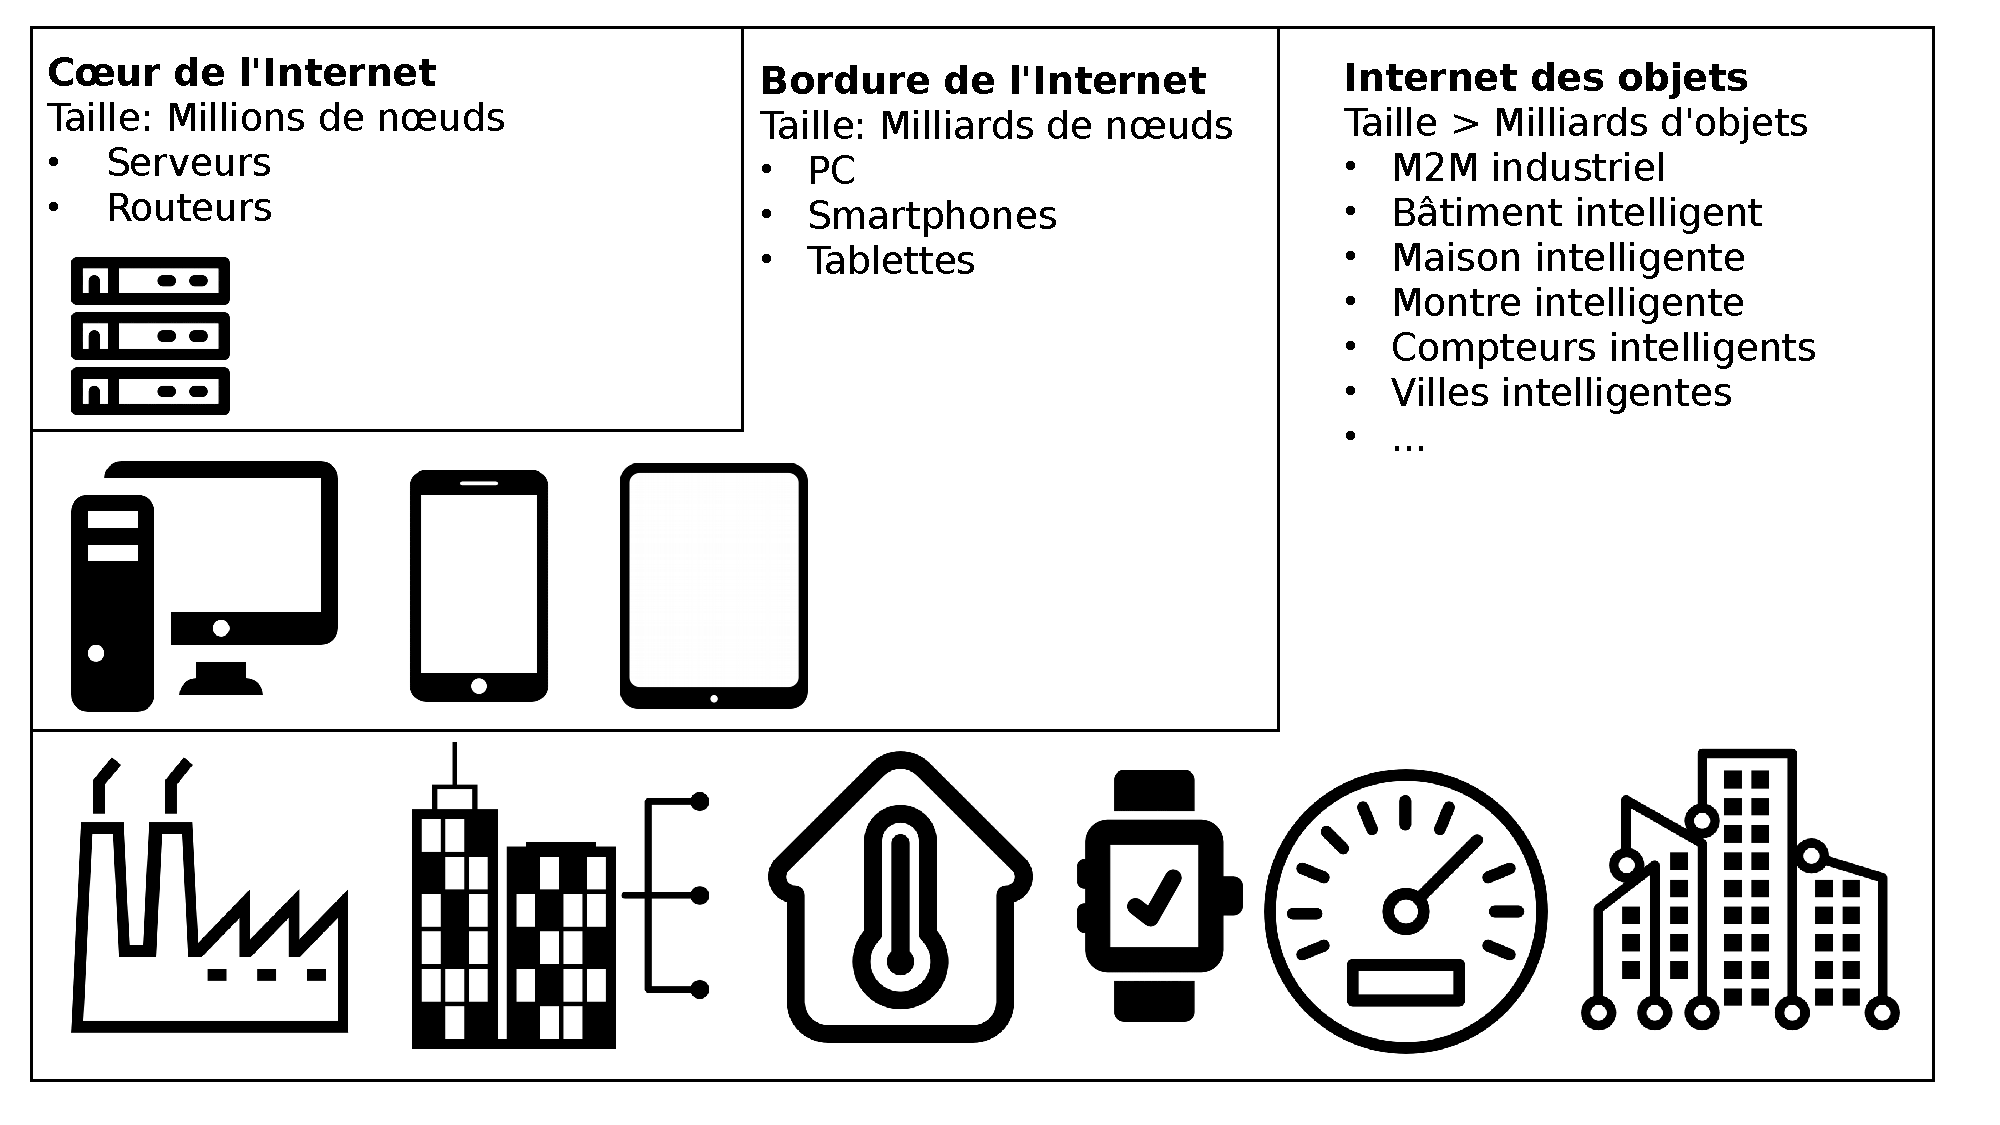
\includegraphics[width=.8\linewidth]{img/iot_vision.pdf}
	\caption{Internet des objets (IoT)}
	\label{intro:iot_vision}
\end{figure}

Internet s'est développé au cours des dernières décennies, partant d'un petit réseau académique pour devenir ubiquitaire et mondial~\cite{pujolle2014reseaux}.
La conception de ce réseau avait pour hypothèses de départ les contraintes technologiques de l'époque: des ordinateurs, toujours connectés, alimentés en énergie en permanence et disposant d'assez de capacité pour gérer le trafic réseau reçu.
L'augmentation croissante du nombre d'appareils connectés comme des ordinateurs, tablettes ou smartphones est venue s'ajouter autour des réseaux de cœur pour l'étendre et proposer de nombreux usages plus mobiles et orientés vers les utilisateurs finaux apportant services et fonctionnalités~\cite{falaki2010diversity}.

L'Internet des objets (appelé \ac{IoT} en anglais) se construit autour des réseaux préexistants montrés sur la Figure~\ref{intro:iot_vision} et vient ajouter à des objets existants des fonctionnalités de connectivité à l'Internet.
L'objectif de l'\ac{IoT} consiste à ajouter une connectivité à Internet pour un coût négligeable à des objets afin de permettre l'émergence de nouveaux services et de simplifier leur utilisation.
Cette tendance est rendue possible par la réduction constante des besoins énergétiques, de la taille, du prix et du poids des processeurs et des capteurs qui a permis d'ajouter une connectivité sans fil à un grand nombre d'appareils~\cite{koomey2011implications}.
Le nombre de machines et leur versatilité sont en pleine croissance~\cite{gubbi2013internet} de même que les marchés pour ces appareils aussi bien dans le secteur privé que grand public.
Les domaines d'applications étant vastes il s'en suit que les applications proposées seront très diversifiées et toucheront l'ensemble de la société.

Pour fonctionner, l'\ac{IoT} repose sur des capteurs envoyant des informations sur leur environnement en temps réel vers des services à valeur ajoutée que les utilisateurs finaux consultent.
Certains de ces capteurs seront intégrés dans des systèmes embarqués devant fonctionner de manière fiable sur de grandes périodes, mais avec des ressources matérielles faibles et des batteries limitées.
Afin d'augmenter leur couverture réseau, ces systèmes sont connectés les uns aux autres pour former des réseaux maillés.
À l'interface de ces réseaux maillés et des réseaux usuels se trouve une passerelle dont l'objectif est de masquer l’hétérogénéité de ces nœuds et leurs contraintes spécifiques tout en leur offrant une connectivité native au reste du réseau.

L'objectif de cette thèse est d'étudier les fonctionnalités que l'interface entre un réseau de capteurs et un réseau conventionnel peut offrir afin d'améliorer les performances et la fiabilité de fonctionnement du réseau visé visé.


Ce chapitre introductif commence par introduire une taxonomie des machines étudiées (\ref{intro:taxonomy}) puis rappelle les enjeux et domaines d'application (\ref{intro:motivations}) et les défis apportés par cette nouvelle tendance (\ref{intro:challenges}).
Les contributions de cette thèse (\ref{intro:contributions}) et le plan (\ref{intro:thesis_outline}) seront ensuite présentés.

\section{Taxonomie des machines en \ac{IoT}}
\label{intro:taxonomy}

\begin{figure}[ht]
  \centering
  \begin{tikzpicture}

  % définition des styles
  \tikzstyle{visible}=[draw, fill=blue!50]
  \tikzstyle{hidden}=[ draw, fill=gray!20]
  \tikzstyle{router}=[circle, draw, fill=orange!50,text=black]
  \tikzstyle{child}=[circle, draw, fill=yellow!50,text=black]
  \tikzstyle{root}=[circle, draw, fill=red!50,text=black]

  

  % Réseau contraint
  \node[root] (LBR) at (-4, 0) {};
  \node[router] (2) at (-5, 1) {};
  \node[child] (3) at (-5, -1) {};
  \node[child] (4) at (-6, 2) {};
  \node[child] (5) at (-6, 0) {};

% les nœuds
  \node[draw, right=of LBR] (gw) {Passerelle};


  % \node[cloud, cloud puffs = 10, minimum width = 4cm, draw, fill = gray!10] (cloud) at (5,0) {Réseau local};
  \node[draw, cloud, cloud puffs = 10, minimum width = 3cm, draw, fill = gray!10, right=of gw] (cloud) {Réseau};
  \node[draw, right=of cloud,] (service) {Services};
  \node[draw, right=of service] (users) {Utilisateurs};  


 \node [fit=(LBR) (2) (3) (4) (5), rounded corners, draw=black!50] (lln) {};
 \node [below=.3 cm of lln] {LLN (Nœuds capteurs)};

\path

  % Réseau contraint
  (gw.west) edge[<->, very thick]  (LBR) 
  % (gw.west) edge[->, thick, bend right=20]  (LBR) 
  (LBR) edge[<->] (2)
  (LBR) edge[<->] (3)
  (2) edge[<->] (4)
  (2) edge[<->] (5)

  % Réseau conventionnel
  (gw.east) edge[<->, very thick,] (cloud.west)
  (cloud.east) edge[<->, very thick] (service.west)
  (service.east) edge[<->, very thick] (users.west)

  ;

  \end{tikzpicture}
  
  \caption{Taxonomie des différents nœuds}
  
  \label{intro:fig:taxonomie}
\end{figure}



Un réseau de capteurs (aussi désigné sous le terme plus spécifique de \ac{LLN} en anglais) désigne un  réseau formé par des capteurs et une passerelle communiquant entre eux sur des connexions radio particulièrement bruitées~\cite{gubbi2013internet}.
Certains de ces nœuds ont un rôle de routeur interne relayant les communications des autres nœuds vers la passerelle (aussi appelé routeur de bordure) afin d'augmenter la couverture d'un réseau sans augmenter les portées de transmission.
C'est ce type de réseau qui est considéré dans cette thèse.

\subsection{Nœuds capteurs}

Afin de mesurer l'environnement et d'interagir avec lui, il est nécessaire d'avoir des capteurs et actionneurs simples, représentés à gauche sur la Figure~\ref{intro:fig:taxonomie}.
Ils sont utilisés dans des contextes variés et répondent à des besoins hétéroclites~\cite{werner2006deploying}.
Ils transmettent et reçoivent des messages courts comme une mesure d'un capteur ou l'ordre de déclenchement d'un actionneur et doivent fonctionner de manière fiable durant des périodes longues.

Les améliorations technologiques sur les composants sont généralement utilisées pour baisser les coûts de production et d'exploitation, notamment en énergie, plutôt que pour améliorer les performances~\cite{murugesan2008harnessing}, ainsi leurs capacités restent limitées.
Autrement dit, les architectures matérielles sont réduites (processeur, mémoire), la consommation énergétique doit être faible et la batterie doit tenir sur de longues périodes~\cite{werner2006deploying}.
Pour qu'ils puissent avoir une grande durée de vie avec des batteries simples (piles classiques) les nœuds se mettent en veille autant que possible pour préserver leurs réserves d'énergie.

Afin de masquer l'hétérogénéité des nœuds et des protocoles spécifiques qu'ils utilisent pour se parler, ces nœuds ont besoin de passerelles pour communiquer avec l'extérieur.

\subsection{Passerelles}

Ces passerelles (parfois aussi appelée routeur de bordure) sont en charge de concilier un écosystème d'appareils hétérogènes, de collecter les données des nœuds capteurs et d'offrir une interface vers eux.
La nature hétérogène des capteurs conduit les passerelles à supporter différents types d'interfaces (par exemple: \ac{CPL}, Bluetooth, cellulaire ou encore Wifi) et protocoles réseau.
Elles masquent ainsi la spécificité des capteurs derrière une interface présentant les ressources avec un formalisme commun.

Les passerelles sont plus performantes que les nœuds capteurs et ont un rôle de médiateur entre différentes technologies, comme montré sur la Figure~\ref{intro:fig:taxonomie} .
Du fait de leur position, les passerelles disposent de beaucoup d'informations sur les nœuds capteurs et peuvent en tirer parti entre autres pour établir et optimiser des tables de routage~\cite{rfc6550} ou découvrir les services offerts par les capteurs~\cite{cirani2014scalable}.
Ces fonctionnalités peuvent s'ajouter à d'autres fonctions (Pare-feux, supervision) et seront détaillées dans le chapitre~\ref{gw}.

\subsection{Infrastructure de services}

Bien que les passerelles assurent la connectivité vers les nœuds, l'intégration de ces données est faite au niveau de serveurs distants~\cite{anton2014machine, atzori2010internet} pour faciliter le passage à l'échelle de sources d'informations multiples.
Ces serveurs peuvent être physiquement localisés dans un même réseau (par exemple dans les scénarios domotique) ou bien chez un fournisseur de services tiers pour en simplifier l'usage (accès depuis l'extérieur, fiabilité renforcée, etc.)
Ils sont représentés à droite sur la Figure~\ref{intro:fig:taxonomie} et représentent le dernier chaînon avant l'utilisateur.
On y trouve les services à valeur ajoutée en charge de traiter, analyser et visualiser les données dans une interface destinée aux consommateurs et utilisateurs finaux.

Il devient alors possible de construire des services basés sur les données collectées en temps réel comme des bulletins météo ou des prévisions de trafic routier \cite{hart2006environmental, gubbi2013internet}.
Dans cette architecture, ces fonctions d'intégration seront au plus proche des utilisateurs finaux afin que seul les alarmes, exceptions ou notifications pertinentes soient envoyées.

\section{Enjeux \& motivations}
\label{intro:motivations}

L'objectif des \ac{LLN}s consiste à offrir en temps réel des mesures et des relevés sur un grand nombre d'objets avec plus d'aisance de déploiement que ce qu'un système filaire classique peut offrir.
Déployés à grande échelle, ces capteurs fournissent des mesures régulières et systématiques de l'environnement permettant des prises de décision plus réactives sur un système complexe.
Les \ac{LLN}s sont utilisés dans des contextes très variés~\cite{anton2014machine, atzori2010internet}.
Les sections suivantes présentent plus en détail les deux principaux champs d'application des \ac{LLN}s: l'industrie et la ville intelligente.

\subsection{Applications en milieu industriel}

Les unités de production industrielle ont besoin d'avoir un contrôle et une supervision en temps réel aussi fine que possible sur leurs chaînes de production~\cite{erol2011wireless, gungor2010opportunities}.
Ces déploiements mettent en jeu des capteurs hétérogènes et doivent rapporter en temps réel les événements de manière fiable tout en s'acclimatant à des conditions variées (température, radiation, produits chimiques).
Les canaux de communications utilisés doivent être fiables, bidirectionnels (on doit pouvoir communiquer avec une machine et elle doit pouvoir répondre sans limites), avec des délais courts et des bandes passantes suffisantes pour des messages compacts.

Les systèmes de télémétrie industriels usuels (\ac{SCADA}) proposent une solution à ce problème.
Ils fonctionnent le plus souvent en filaire et dans de grands déploiements cette solution peut être difficile ou coûteuse à mettre en place~\cite{anton2014machine}.
De plus, les interconnexions entre les différents systèmes de télémétrie, qu'elles soient physiques (câble) ou bien logicielles sont très souvent propriétaires, incompatibles avec les machines de la concurrence et aux fonctionnalités limitées et peu évolutives.

Les \ac{LLN}s utilisent des protocoles interopérables et des standards ouverts entre tous les équipements de différents constructeurs ce qui permet de disposer d'une interopérabilité entre des systèmes très hétérogènes~\cite{shelby20116lowpan, walter2009implementing}.
Afin de réduire les coûts d'interopérabilité, on assiste désormais à la croissance des communications \ac{M2M} reposant sur des standards réseau compatibles avec ceux utilisés sur Internet et proposant une normalisation des interfaces applicatives.

\subsubsection{Agriculture et élevage intelligent}

Les exploitations agricoles sont en croissance du point de vue de leur superficie et de leurs productions, elles adoptent de plus en plus des méthodes de production venues du monde industriel~\cite{ruiz2009review}.
Les besoins sont nombreux: surveiller en temps réel l'état des plantations, l’irrigation, la présence de pesticide ou de produits chimiques, l'acidité des sols et des conditions météorologiques~\cite{wark2007transforming}.
Pour ces besoins, il est nécessaire de disposer de méthodes de relevés fiables de l'environnement en temps réel permettant de prendre des décisions de manière automatisée à grande échelle.
Les \ac{LLN}s offrent toutes ces possibilités et permettant par exemple de surveiller l'état de santé d'un animal s'assurer que son état et son environnement sont conformes avec les normes en vigueur et s'assurer de sa traçabilité ainsi que de sa localisation, ce qui rend les contrôles sanitaires plus rapides, fiables et systématiques sur de grandes échelles cela afin d'éviter les intoxications alimentaires~\cite{wang2006wireless}.

\subsubsection{Gestion de bâtiment - Domotique}

La domotique et la gestion de bâtiment sont des secteurs en pleine expansion~\cite{martocci2010building, ehlers1996engery}.
Le but est d'obtenir au sein d'un bâtiment un système pouvant superviser l'état de l'immeuble sur différents critères comme le chauffage, l'air conditionné, la ventilation et l'allumage des pièces, la fermeture des portes ou la détection de cambriolage~\cite{mainwaring2002wireless}.
Le faible coût et la facilité de déploiement des \ac{LLN} permettent de les installer rapidement afin d'améliorer le confort et le contrôle à distance d'un grand bâtiment ou d'une habitation.
Une fois ce contrôle disponible, il est possible de contrôler le chauffage de manière beaucoup plus automatisée sans l'intervention d'un technicien sur le site et de contrôler plus finement la dépense énergétique pour chauffer un bâtiment ce qui peut conduire à des économies importantes~\cite{egan2005emergence}.

\subsection{Applications pour les villes intelligentes}

Les villes deviennent de plus en plus peuplées et la modernisation de leur fonctionnement permet des économies et des gains de qualité de vie pour chacune d'entre elles~\cite{caragliu2011smart}.
La variété des déploiements et des autorités mises en jeu rend ce contexte différent de celui des applications industrielles où une autorité unique prend la décision d'intégrer un nouveau système à l'existant.
Le but de la ville intelligente est de permettre le déploiement de systèmes à l'échelle d'une ville ou d'un territoire afin de faciliter la vie de ses habitants~\cite{hollands2008will}.

\subsubsection{Voirie}

Les villes ont par exemple besoin de pouvoir réduire efficacement le temps passé par un automobiliste pour trouver une place de stationnement dans le but de réduire le carburant utilisé  et limiter les bouchons de circulation.
Les systèmes de Smart parking~\cite{medaglianibringing} sont un bon exemple de déploiement urbain permettant d'avoir en temps réel la disponibilité des places de parking.
Ces systèmes sont mis en place en combinant des capteurs détectant des places disponibles sur la chaussée et envoyant ces informations vers des serveurs qui les redistribuent vers des utilisateurs finaux en temps réel.
La gestion du trafic automobile et des piétons peut également être plus efficace quand le trafic est fluidifié par des feux de circulation qui s'adaptent pour le gérer au mieux~\cite{de1998optimal,faye2012distributed}.

Enfin, ces systèmes ont l'avantage de réduire les coûts de fonctionnement sur des temps courts et peuvent être justifiés facilement par la réduction des dépenses publiques et la qualité de vie améliorée pour les habitants de la ville~\cite{song2014high, lee2013integrated}.

\subsubsection{Sécurité et Urgences}

La surveillance d'infrastructure comme des voies de chemin de fer, des frontières ou bien des convois sont nécessaires afin d'assurer une sûreté de fonctionnement pour les usagers et les biens.
Dans ce genre de situation, les systèmes doivent résister à de nombreuses attaques ou altérations de leur environnement tout en étant capables de répondre en temps réel en cas d'attaque et d'être fiables tout au long du déploiement.
Des systèmes utilisant des \ac{LLN}s sont mis en œuvre dans des cas de protection et de surveillance de zone dangereuses ou sécurisées~\cite{cao2005analysis}.
Elles permettent la rapidité de déploiement sans fil, la mobilité et la détection en temps réel à moindre coût.
Ces approches peuvent être couplées avec celle des villes intelligentes dans le cas de surveillances des ponts, des routes ou de grandes structures par leurs vibrations~\cite{kim2007health} afin de pouvoir altérer le trafic quand une partie de la route n'est pas sure.
En outre, la surveillance systématique des infrastructures permet de détecter des problèmes plus rapidement et efficacement.
Le déploiement des \ac{LLN}s permet d'avoir des relevés en temps réel de ces installations.
Couplé à des actionneurs, il est possible d'effectuer certaines tâches de maintenance à distance et automatiquement et donc d'éviter de solliciter un technicien.

\subsubsection{Environnements intelligents}

Détecter un risque environnemental est une nécessité pour protéger efficacement les populations et l'environnement.
Afin de surveiller en temps réel une large zone, des moyens coûteux (photos satellites, surveillance aérienne, patrouilles) et peu réactifs sont possibles, mais ne sont pas utilisables par les autorités chargées de cette surveillance pour des raisons de coûts ou de logistique.
Les \ac{LLN}s peuvent permettre un suivi en temps réel sur des zones géographiques larges et à moindre coût afin de permettre aux autorités d'intervenir rapidement quand une alerte est déclenchée.
Des déploiements ont déjà été réalisés afin de prévenir des feux de forêt~\cite{yu2005real}, des avalanches et glissements de terrain~\cite{terzis2006slip, alippi2007adaptive}, de permettre la détection des risques sismiques et volcaniques~\cite{werner2006deploying} ou bien la supervision de la qualité de l'eau et de l'air dans des terrains industriels ou contaminés~\cite{khedo2010wireless, o2007smartcoast}.
Les scénarios de surveillance de l'eau~\cite{xiao2010smart}, d'une rivière ou nappe phréatique sont particulièrement pertinent dans le cas de ville ou de zone géographique où l'eau est rare~\cite{kerkez2012design}.

\section{Défis introduits par les \ac{LLN}s}
\label{intro:challenges}

Les \ac{LLN}s sont des réseaux composés de systèmes embarqués caractérisés par une faible consommation énergétique, l'interconnexion native avec Internet via leur passerelle et des ressources limitées sur chaque nœud.
Les systèmes embarqués sont devenus, avec la croissance des smartphones, les appareils majoritaires en nombre sur Internet et cette croissance se maintient dans beaucoup de pays~\cite{kim2007value}.
L'objectif voulu par les \ac{LLN}s est de fournir des mesures en temps réel d'un environnement afin de permettre la création de services autour de ces données mesurées.
Cependant, les \ac{LLN}s disposent de leurs propres défis techniques qui les distinguent des systèmes embarqués usuels comme les smartphones et qui tiennent à leur nature même et à leurs déploiements.

La présentation de ces défis sera découpée en deux axes~: l'un portant sur les défis relatifs aux nœuds et l'autre sur ceux liés à la mise en réseau de ces mêmes nœuds.

\subsection{Défis liés aux nœuds}

Les nœuds capteurs sont des systèmes embarqués visant à fournir des mesures sur leur environnement et à exécuter des actions sur celui-ci~\cite{kopetz2011real}.
Ces nœuds sont composés de capteurs, d'actionneurs et fonctionnent grâce à un microcontrôleur ou bien avec un microprocesseur sur lequel s’exécute un système d'exploitation spécifique~\cite{dunkels2004contiki}.
Ces composants qu'ils soient matériels ou logiciels consomment aussi peu de ressources que possible, visent à être aussi fiables que possible, et cela pour un faible coût de production.
Contrairement à d'autres systèmes embarqués comme des smartphones, ils ne cherchent pas à être des systèmes universels ni à devenir plus performants.
Les évolutions technologiques visent à réduire leur coût et améliorer leur efficacité énergétique~\cite{koomey2011implications}.
En plus de ces contraintes spécifiques, d'autres défis viennent s'ajouter lorsque ces capteurs sont déployés dans le contexte spécifique des \ac{LLN}s.

\subsubsection{Hétérogénéité technologique et fonctionnelle}

%Pourquoi c'est important
Le grand nombre de constructeurs impliqués dans les \ac{LLN}s et la multitude des domaines d'applications a conduit à l'émergence de plusieurs standards~\cite{bandyopadhyay2011internet}.
Orchestrer un écosystème hétérogène tant en terme de domaines d'applications que de choix technologiques est donc un défi complexe à réaliser.

%Pourquoi c'est difficile
L'hétérogénéité se situe à plusieurs niveaux~: segments (grand public, industriel), chaînes de valeur (opérateur, fournisseur de service), délais de standardisation (time to market), taille du segment et influence géographique.
Cela fait que de nombreux standards coexistent et que des outils seront requis pour offrir des interfaces entre ces différents standards.
Des organismes nationaux et internationaux se penchent sur les questions d'interopérabilité et de standardisation~: Allseen Alliance, Industrial Internet Consortium, ETSI, Open Interconnect, Thread, IPSO Alliance, IEEE\ldots

\subsubsection{Cycle de vie}

%Pourquoi c'est important
Les fonctions d'un nœud capteur peuvent changer et nécessiter des mises à jour logicielles par exemple pour corriger des failles de sécurité ou ajouter de nouvelles fonctionnalités.
Un déploiement rapide des correctifs et des mises à jour est un facteur clé pour éviter l’obsolescence d'un objet connecté et les problèmes de sécurité qui en découlent~\cite{pathan2006security, wang2006survey}.

%Pourquoi c'est difficile
Toutefois, il peut être difficile de mettre à jour, par exemple quand le déploiement a lieu dans un terrain difficile d'accès comme un volcan ou une zone de montagne.
Des solutions de migrations, de maintenance et de déploiement d'applications à distance sont donc requises~\cite{brown2006updating, stathopoulos2003remote}.

\subsection{Défis liés au réseau}

Les nœuds capteurs disposent d'une faible capacité d'émission radio, ainsi les mettre en réseau afin qu'ils communiquent entre eux vers une passerelle permet d'améliorer la couverture du réseau tout en maintenant des portées de transmissions faibles.
Cependant la mise en réseau des \ac{LLN}s comporte des défis techniques.

\subsubsection{Pertes}

Les \ac{LLN}s utilisent généralement des bandes de fréquences libres (\ac{ISM}) pour communiquer afin d'éviter les coûts d'une licence pour une fréquence propre.
Les canaux étant communs, les liens sont bruités, instables et les pertes de paquets sont donc courantes~\cite{baccour2012radio}.
De plus, les capteurs émettent avec une faible puissance pour économiser de l'énergie ainsi ils sont particulièrement sensibles aux conditions du canal et leur signal peut être écrasé par d'autres signaux émis dans la même bande de fréquence comme du Wi-Fi.
En outre des phénomènes d’atténuation dus à la réverbération (Multipath fading) se produisent et perturbent les communications mêmes si elles sont à portée de transmission \cite{puccinelli2006multipath}.

%Pourquoi c'est important

En cas de trop fortes pertes et de conditions trop instables sur le réseau, les \ac{LLN}s peuvent adapter la topologie de routage utilisée pour communiquer plus efficacement avec la passerelle~\cite{clausen2011critical}.
Ceci peut provoquer des reconfigurations dans tout le \ac{LLN}, ainsi des mécanismes doivent être mis en place dans les protocoles pour garantir la connectivité et la fiabilité des communications entre les capteurs et la passerelle à moindre coût énergétique~\cite{6tisch}.

\subsubsection{Connexions intermittentes}

%Pourquoi c'est important
Afin d'économiser autant d'énergie et de bande passante que possible, les nœuds se mettent en sommeil régulièrement.
Durant cette période, leur consommation énergétique est significativement inférieure à la moyenne, mais le nœud est alors difficilement joignable~\cite{kellner2008towards}.
Cela entraîne l'intermittence des liaisons radio entre chaque nœud~\cite{duarte2002analysis} et implique qu'il est particulièrement difficile de savoir si un nœud est en panne, indisponible ou endormi dans le cas où ces cycles de sommeil ne sont pas déterministes.
Les appareils doivent donc gérer eux-mêmes les confirmations et la fiabilité des transmissions, car utiliser un protocole de transport classique apporterait trop de surcoûts en entêtes et retransmissions~\cite{rfc7252}.
Ainsi des protocoles sans sessions et des architectures robustes aux déconnexions sont privilégiés afin de transmettre des messages dans le \ac{LLN}.

%Pourquoi c'est difficile
% Dans le cas où les cycles d'endormissements sont gérés par une autorité centrale, il est nécessaire d'introduire une signalisation supplémentaire afin de gérer les cycles d'activité et d'utilisation du canal~\cite{6tisch}.
% Si chaque noeud gère son propre cycle d'endormissement indépendament des autres noeuds, les sources doivent émettre les messages plusieurs fois pour qu'il puisse être eventuellement reçu~\cite{dunkels11contikimac}.
% Enfin quelque soit le mécanisme d'endormissement utilisé, il existe des attaques au déni de sommeil empêchent les nœuds de dormir et use leurs ressources déjà limitées pour rendre à terme le réseau indisponible~\cite{raymond2008denial}.

\subsubsection{Besoin de protocoles optimisés}

%Pourquoi c'est important
Dans les déploiements classiques des \ac{LLN}s, les quantités de données échangées sont très réduites et intermittentes afin de préserver l'énergie~\cite{tan2010future}.
Cela requiert d'utiliser des protocoles spécifiques (compact, sans maintien d'état, avec des entêtes compressés) qui réduisent leur impact autant que faire se peut~\cite{Winter2012,shelby20116lowpan,rfc6690}.

%Pourquoi c'est difficile
Les protocoles classiques utilisés dans l'état de l'art pour faire fonctionner l'Internet ont été conçus pour des appareils étant toujours allumés, générant un trafic important et en croissance.
En outre, utiliser les protocoles classiques occuperait une quantité importante de la bande passante et engendrerait donc un surcoût non négligeable de consommation d'énergie.
L'émergence de ces protocoles justifie l'apparition d'une couche applicative d'interopérabilité afin d'orchestrer les différents nœuds sans se focaliser sur leurs spécificités~\cite{van2008achieving}.

\subsubsection{Écoute passive en zone dense}

%Pourquoi c'est important
De nombreux protocoles d'accès utilisés dans les \ac{LLN}s sont asynchrones afin d'éviter de mettre en place une signalisation régulière coûteuse en énergie et en bande passante sur chaque nœud.
Lorsqu'un nœud reçoit un signal asynchrone, il doit le décoder et l'analyser afin de décider si cette transmission lui est destinée et si une tâche doit être accomplie.
Ce décodage systématique a un coût élevé dans des environnements denses~\cite{langendoen2008medium}.

%Pourquoi c'est difficile
%Eventuels renvois(Etat de l'art/section de la thèse)

Ainsi pour des déploiements denses avec un grand nombre de nœuds, il est indispensable d'utiliser des protocoles spécifiques permettant d'avoir aussi bien passage à l'échelle en nombre de nœuds que consommation énergétique minimale lors du décodage des trames émises~\cite{6tisch}.
Les phénomènes de capture typiques de l'écoute passive sont donc évités et l'énergie n'est utilisée que pour décoder des messages pertinents pour le nœud.

\subsubsection{Passage à l'échelle}

%Pourquoi c'est important
La croissance du nombre d'appareils connectés à Internet reste forte et l'ajout des nœuds venant des \ac{LLN}s ne fera qu'accentuer cette croissance, car la baisse continue des coûts de production conduit à des nœuds toujours plus nombreux et moins cher~\cite{tan2010future, loomis2012forecasting}.
Cela pose la question du passage à l'échelle de ce type d'installation dans des réseaux qui peuvent déjà être chargés~\cite{murugesan2008harnessing,brownlee2002understanding,bandyopadhyay2011internet}.
La question du passage à l'échelle concerne à la fois la coordination des nœuds, le partage de leurs ressources et les besoins d'adressage.

Afin de répondre à un besoin croissant d'adressage, IPv6 a été introduit afin de fournir un espace d'adressage global suffisant.
L'émergence des \ac{LLN}s rend IPv6 encore plus pertinent, car il permet de disposer d'un adressage complet de tous les nœuds sur un réseau commun qu'il soit global ou privé sans utiliser de mécanisme intermédiaire coûteux comme un mécanisme de traduction d'adresse réseau (\ac{NAT}).
Cette identification unique permet de facilement fournir une communication sans intermédiaire et simplifie la gestion du réseau par un formalisme commun.
De plus, des mécanismes de compression d'IPv6 sont disponibles afin de bénéficier de l'espace d'adressage tout en limitant la taille des entêtes utilisés.

% \subsubsection{Fragmentation}

% La fragmentation arrive lorsqu'un paquet plus grand que la \ac{MTU} est transmis~\cite{shelby20116lowpan}.
% Ce type de problème peut arriver en \ieee{} où les paquets sont limités à 127 octets~\cite{ludovici2011forwarding}.
% La fragmentation peut également donner lieu à des attaques où les nœuds surchargent leur mémoire avec des paquets intermédiaires et non reconstitués~\cite{hummen20136lowpan}.

% \subsubsection{Mobilité}

% La mobilité des nœuds peut entraîner des pertes de connectivité, des reconfigurations de topologie réseau et des congestions~\cite{lee2012rpl}.
% Dans le cas des \ac{BAN}, le réseau entier peut être mobile~\cite{chen2011body} et gérer des connexions/deconnexions régulièrement.
% Des mécanismes de découvertes de voisins et de topologies peuvent permettre de gérer les cas de mobilité au sein d'un même \ac{LoWPAN}~\cite{oliveira2011routing}.

\section{Aperçu des contributions}
\label{intro:contributions}

La passerelle jour un rôle clé dans la mesure, car elle interface le \ac{LLN} avec le reste du réseau.
Elle sert de médiateur et traite donc la problématique de l'interopérabilité des nœuds et des différentes contraintes des capteurs.
Sa position dans le réseau lui permet en outre d'avoir une vue précise du \ac{LLN} et des informations qui y rentrent et en sortent.

Le but de cette thèse est d'exposer comment des fonctionnalités peuvent être ajoutées à l'interface d'un \ac{LLN} et du reste du réseau pour améliorer l'utilisation des ressources et la connaissance de l'état du \ac{LLN}.
Les contributions proposées dans cette thèse ont pour objectif d'améliorer les performances et la fiabilité d'un \ac{LLN}.


\subsection{Mesure implicite de la consommation énergétique d'un \ac{LLN}}

% \subsubsection{Description du problème}

Pour s'assurer que le fonctionnement d'une application est correct, un administrateur a besoin de connaître l'état des nœuds du \ac{LLN} dont dépend son application.
Préserver l'énergie consommée est un problème clé pour ce type de réseau.
Il parait donc naturel de mettre à disposition des administrateurs un moyen peu consommateur d'énergie leur permettant d'estimer l'état de leur réseau, d'obtenir une durée de vie estimée et connaître les nœuds les plus sollicités dans une topologie multi sauts.

% \subsubsection{Limites de l'état de l'art}

Mesurer explicitement ces informations n'est pas toujours possible et même quand c'est le cas, il est coûteux de le demander à chaque nœud dans un réseau de grande taille.
Ainsi des approches induisant un minimum de transmissions de données peuvent aider à obtenir une cartographie de la consommation énergétique et de l'utilisation de la radio à moindre coût.

% \subsubsection{Contributions}

Le chapitre~\ref{supervision} montre comment l'observation du trafic routé passant par la passerelle permet d'inférer l'utilisation de la radio, et, dans une certaine mesure, la consommation énergétique.
Les limites de cette approche seront également décrites et une correction des biais sera proposée lorsque la supervision active est possible.

\subsection{Optimisation des ressources du \ac{LLN} avec un cache intelligent}

% \subsubsection{Description du problème}
La passerelle offre une interface vers le \ac{LLN} et reçoit les requêtes applicatives qui lui sont destinées.
Le traitement d'une requête par le \ac{LLN} est lent, car les nœuds sont peu performants.
De plus chaque requête consomme de l'énergie qui est une ressource limitée.
Ainsi la passerelle a pour objectif de solliciter le \ac{LLN} aussi peu que possible tout en répondant de manière fiable aux requêtes.

% \subsubsection{Limites de l'état de l'art}

Une stratégie usuelle pour accélérer les réponses et économiser de l'énergie consiste à maintenir dans un cache au niveau de la passerelle la réponse à une requête donnée pendant un temps de validité précis.
Ainsi si la passerelle dispose d'une réponse encore valide pour une requête donnée, elle l'utilise au lieu de solliciter le \ac{LLN}.
Déterminer le temps de validité d'une réponse pour chaque ressource doit tenir compte de multiples paramètres et la littérature n'offre pas de méthode explicite pour déterminer des temps de validité efficace pour une configuration donnée.

% \subsubsection{Contributions}

Le chapitre~\ref{cache} propose de déterminer les temps de validité pour réguler le trafic entrant vers les nœuds du \ac{LLN} en fonction de la durée de vie des nœuds visée par l'administrateur et fraîcheur des réponses attendues.
Les objectifs étant antagonistes, il est nécessaire de procéder à un arbitrage afin de trouver un compromis entre différentes solutions.
Une modélisation donnée sous la forme d'une optimisation multi-objectifs permettra de fournir un ensemble de solutions admissibles optimales.

\subsection{Expériences automatisées et reproductibles pour \ac{LLN}s}

% \subsubsection{Description du problème}

Effectuer une expérience avec des \ac{LLN}s met en jeu de nombreux logiciels et des procédures qui sont longues et fastidieuses lorsqu'elles sont réalisées manuellement.
Cela rend une expérience difficile à reproduire surtout si elle n'est pas ré-effectuée par la ou les mêmes personnes.
Lorsque de nombreuses étapes sont nécessaires pour obtenir un résultat, documenter et automatiser l'expérience en question autant que possible devient crucial afin qu'elle puisse être reproduite et validée par la communauté scientifique et de s'assurer de leur véracité efficacement.

% \subsubsection{Limites de l'état de l'art}

Les bancs de test (appelés testbeds en anglais) prévus pour les \ac{LLN}s fournissent de nombreux outils dédiés au lancement d'expériences et à la collecte de résultats~\cite{buchert2015survey,fleury2015fit}.
Cependant il n'existe pas de solution complète pour lancer, récupérer et exploiter les données issues d'expériences et de simulations dans un seul outil cohérent et intégré.
En outre, l'un des écueils à éviter lors de la conception de tels outils est de définir une architecture trop spécialisée et donc inutilisable dans d'autres contextes ce qui limiterait d'emblée son impact.

% \subsubsection{Contributions}

Le chapitre~\ref{makesense} propose un framework d'organisation d'expérience permettant de documenter, d'exécuter et d'analyser l'ensemble d'une expérience sur \ac{LLN}.
Fonctionnant à la fois en simulation et sur nœuds réels, Makesense permet d'obtenir un framework d'expériences reproductibles.
Ce chapitre consacré à Makesense illustrera son fonctionnement au travers d'une expérience typique.
Il présente entre outre les étapes clés d'une expérience et montre que les choix technologiques ne requièrent pas une implémentation spécifique, mais utilise au contraire des outils classiques et largement utilisés par la communauté scientifique.
Enfin, un mécanisme d'intégration continue automatisera l'expérience et apportera ainsi la preuve de sa reproductibilité.

\subsection{Collaborations extérieures faites durant la thèse}

Un aperçu des collaborations extérieures effectuées au long de cette thèse avec des chercheurs extérieurs à notre équipe de recherche est disponible en annexe~\ref{collaborations}.

\section{Plan du manuscrit}
\label{intro:thesis_outline}

Les contributions de cette thèse exposent différentes fonctionnalités et améliorations que la passerelle peut offrir afin d'améliorer les performances et la fiabilité de ces réseaux.

Le chapitre~\ref{gw} introduit plus en détail les \ac{LLN}s.
Il présente les hypothèses de travail et les choix faits dans cette thèse pour interfacer un \ac{LLN} avec d'autres réseaux et les confronte avec ceux couramment trouvés dans la littérature.

Le chapitre~\ref{supervision} montre comment la mesure des temps d'utilisation de la radio dans un \ac{LLN} permet de prévoir la consommation énergétique implicitement.

Le chapitre~\ref{cache} expose comment l'utilisation d'un cache applicatif peut être adapté pour optimiser l'utilisation des ressources d'un \ac{LLN} en modifiant les temps de validité des réponses des requêtes qu'il reçoit.

Le chapitre~\ref{makesense} présente Makesense le framework d'expérimentation utilisé ultérieurement dans les chapitres~\ref{cache} et \ref{supervision} pour documenter, reproduire et partager les expériences effectuées sur les \ac{LLN}s.

Enfin, le chapitre~\ref{conclusion} conclue cette thèse et ouvre sur des prolongements possibles.

% L'annexe~\ref{contikimac} présentera une modélisation de ContikiMAC,
% Des extraits de code utilisés par Makesense seront présentés dans l'annexe~\ref{code} et 
L'annexe~\ref{collaborations} présentera les collaborations extérieures faites pendant cette thèse et présentera les publications obtenues.


\cleardoublepage % Empty page before the start of the next part

%------------------------------------------------

\ctparttext{You can put some informational part preamble text here. Illo
principalmente su nos. Non message \emph{occidental} angloromanic da. Debitas
effortio simplificate sia se, auxiliar summarios da que, se avantiate
publicationes via. Pan in terra summarios, capital interlingua se que. Al via
multo esser specimen, campo responder que da. Le usate medical addresses pro,
europa origine sanctificate nos se.}

\part{The Showcase} % Second part of the thesis

% Chapter 2

\chapter{Examples} % Chapter title

\label{ch:examples} % For referencing the chapter elsewhere, use \autoref{ch:examples} 

\graffito{Note: The content of this chapter is just some dummy text.}

%------------------------------------------------

\subsection{Personas Initialmente}

\lipsum[10]

\subsubsection{A Subsubsection}
\lipsum[11]

\paragraph{A Paragraph Example} \lipsum[12]

\begin{aenumerate}
\item Enumeration with small caps
\item Second item
\item Second item
\end{aenumerate}

\noindent Another statement requiring citation \cite{sommerville:1992} \cite{sommerville:1992} but this time with text after the citation.

%\begin{table}
%\myfloatalign
%\begin{tabularx}{\textwidth}{Xll} \toprule
%\tableheadline{labitur bonorum pri no} & \tableheadline{que vista}
%& \tableheadline{human} \\ \midrule
%fastidii ea ius & germano &  demonstratea \\
%suscipit instructior & titulo & personas \\
%\midrule
%quaestio philosophia & facto & demonstrated \citeauthor{knuth:1976} \\
%\bottomrule
%\end{tabularx}
%\caption[Autem timeam deleniti usu id]{Autem timeam deleniti usu id. \citeauthor{knuth:1976}}  
%\label{tab:example}
%\end{table}

\enlargethispage{2cm}

%------------------------------------------------

\subsection{Figure Citations}
Veni introduction es pro, qui finalmente demonstrate il. E tamben anglese programma uno. Sed le debitas demonstrate. Non russo existe o, facite linguistic registrate se nos. Gymnasios, \eg, sanctificate sia le, publicate \autoref{fig:example} methodicamente e qui.

Lo sed apprende instruite. Que altere responder su, pan ma, \ie, signo studio. \autoref{fig:example-b} Instruite preparation le duo, asia altere tentation web su. Via unic facto rapide de, iste questiones methodicamente o uno, nos al.

%\begin{figure}[bth]
%\myfloatalign
%\subfloat[Asia personas duo.]
%{\includegraphics[width=.45\linewidth]{gfx/example_1}} \quad
%\subfloat[Pan ma signo.]
%{\label{fig:example-b}
%\includegraphics[width=.45\linewidth]{gfx/example_2}} \\
%\subfloat[Methodicamente o uno.]
%{\includegraphics[width=.45\linewidth]{gfx/example_3}} \quad
%\subfloat[Titulo debitas.]
%{\includegraphics[width=.45\linewidth]{gfx/example_4}}
%\caption[Tu duo titulo debitas latente]{Tu duo titulo debitas latente.}\label{fig:example}
%\end{figure}
 % Chapter 2

%----------------------------------------------------------------------------------------
%	THESIS CONTENT - APPENDICES
%----------------------------------------------------------------------------------------

% \appendix

% \part{Appendix} % New part of the thesis for the appendix

% \include{tex/Chapter0A} % Appendix A
%\include{tex/Chapter0B} % Appendix B - empty template

%----------------------------------------------------------------------------------------
%	POST-CONTENT THESIS PAGES
%----------------------------------------------------------------------------------------

\cleardoublepage% Bibliography

\label{app:bibliography} % Reference the bibliography elsewhere with \autoref{app:bibliography}

\manualmark
\markboth{\spacedlowsmallcaps{\bibname}}{\spacedlowsmallcaps{\bibname}} 
\refstepcounter{dummy}

\addtocontents{toc}{\protect\vspace{\beforebibskip}} % Place the bibliography slightly below the rest of the document content in the table of contents
\addcontentsline{toc}{chapter}{\tocEntry{\bibname}}

\bibliographystyle{plain}
\bibliography{main}

%\bibliographystylemine{plain}
%\bibliographymine{mine}
 % Bibliography

\cleardoublepage% Colophon (a brief description of publication or production notes relevant to the edition)

\pagestyle{empty}

\hfill

\vfill

\pdfbookmark[0]{Colophon}{colophon}

\section*{Colophon}

This document was typeset using the typographical look-and-feel
\texttt{classicthesis} developed by André Miede. The style was inspired by
Robert Bringhurst's seminal book on typography ``\emph{The Elements of
Typographic Style}''.
 % Colophon


\cleardoublepage%\usepackage[left=1.3cm,top=0cm,right=1.3cm,bottom=1.2cm]{geometry}

% \usepackage{array}
% \usepackage{textcomp}
% \usepackage{helvet}	% or \usepackage{lmodern}
% \renewcommand\textnumero{n$^{\textsf{{\tiny O}}}$}
% \renewcommand{\familydefault}{\sfdefault}

\newgeometry{left=1.3cm,top=1cm,right=1.3cm,bottom=1.2cm}

\pagestyle{empty}

\AddToShipoutPicture*{\BackgroundPicLastPage}

\vspace{1.5cm}


\begin{center}{\LARGE \textbf{\myTitle}}\\
\vspace{.4cm}
{\large \textbf{\myName}}\\
\end{center}

\vspace{.9cm}

\textbf{RESUME :}

Lorem ipsum dolor sit amet, consectetur adipisicing elit, sed do eiusmod
tempor incididunt ut labore et dolore magna aliqua. Ut enim ad minim veniam,
quis nostrud exercitation ullamco laboris nisi ut aliquip ex ea commodo
consequat. Duis aute irure dolor in reprehenderit in voluptate velit esse
cillum dolore eu fugiat nulla pariatur. Excepteur sint occaecat cupidatat non
proident, sunt in culpa qui officia deserunt mollit anim id est laborum.

Lorem ipsum dolor sit amet, consectetur adipisicing elit, sed do eiusmod
tempor incididunt ut labore et dolore magna aliqua. Ut enim ad minim veniam,
quis nostrud exercitation ullamco laboris nisi ut aliquip ex ea commodo
consequat. Duis aute irure dolor in reprehenderit in voluptate velit esse
cillum dolore eu fugiat nulla pariatur. Excepteur sint occaecat cupidatat non
proident, sunt in culpa qui officia deserunt mollit anim id est laborum.

\vspace{.6cm}

\textbf{MOTS-CLEFS:}  bla bla bla 

\vspace{1.0cm}

\textbf{ABSTRACT:} 

Lorem ipsum dolor sit amet, consectetur adipisicing elit, sed do eiusmod
tempor incididunt ut labore et dolore magna aliqua. Ut enim ad minim veniam,
quis nostrud exercitation ullamco laboris nisi ut aliquip ex ea commodo
consequat. Duis aute irure dolor in reprehenderit in voluptate velit esse
cillum dolore eu fugiat nulla pariatur. Excepteur sint occaecat cupidatat non
proident, sunt in culpa qui officia deserunt mollit anim id est laborum.

Lorem ipsum dolor sit amet, consectetur adipisicing elit, sed do eiusmod
tempor incididunt ut labore et dolore magna aliqua. Ut enim ad minim veniam,
quis nostrud exercitation ullamco laboris nisi ut aliquip ex ea commodo
consequat. Duis aute irure dolor in reprehenderit in voluptate velit esse
cillum dolore eu fugiat nulla pariatur. Excepteur sint occaecat cupidatat non
proident, sunt in culpa qui officia deserunt mollit anim id est laborum.

\vspace{.6cm}
\textbf{KEY-WORDS: } bla bla bla

\restoregeometry

% \cleardoublepage% Declaration

\refstepcounter{dummy}
\pdfbookmark[0]{Declaration}{declaration} % Bookmark name visible in a PDF viewer

\chapter*{Declaration} % Declaration section text

\thispagestyle{empty}

Put your declaration here.
\bigskip
 
\noindent\textit{\myLocation, \myTime}

\smallskip

\begin{flushright}
\begin{tabular}{m{5cm}}
\\ \hline
\centering\myName, \today \\
\end{tabular}
\end{flushright}
 % Declaration

%----------------------------------------------------------------------------------------

\end{document}
